%%=====================================================================================
%%
%%       Filename:  data-structs-and-algs.tex
%%
%%    Description:  Formal notes of DS and A
%%
%%        Version:  1.0
%%        Created:  02/10/19
%%       Revision:  none
%%
%%         Author:  Josh Felmeden (), nk18044@bristol.ac.uk
%%   Organization:  
%%      Copyright:  Copyright (c) 2019, Josh Felmeden
%%
%%          Notes:  
%%
%%=====================================================================================

% Preamble {{{
\documentclass[11pt,a4paper,titlepage,dvipsnames,cmyk]{scrartcl}
\usepackage[english]{babel}
\typearea{12}
% }}}

% Set indentation and line skip for paragraph {{{
\setlength{\parindent}{0em}
\setlength{\parskip}{1em}
\usepackage[margin=2cm]{geometry}
\addtolength{\textheight}{-1in}
\setlength{\headsep}{.5in}
% }}}

\usepackage{hhline} 
\usepackage{mathtools} 
\usepackage[T1]{fontenc}

% Headers setup {{{
\usepackage{fancyhdr}
\pagestyle{fancy}
\lhead{Data Structures and Algorithms: The formal notes}
\rhead{Josh Felmeden}
\usepackage{hyperref} 
% }}}

% Listings {{{
\usepackage[]{listings,xcolor} 
\lstset
{
    breaklines=true,
    tabsize=3,
    showstringspaces=false
}

\definecolor{lstgrey}{rgb}{0.05,0.05,0.05}
\usepackage{listings}
\makeatletter
\lstset{language=[Visual]Basic,
    backgroundcolor=\color{lstgrey},
    frame=single,
    xleftmargin=0.7cm,
    frame=tlbr, framesep=0.2cm, framerule=0pt,
    basicstyle=\lst@ifdisplaystyle\color{white}\footnotesize\ttfamily\else\color{black}\footnotesize\ttfamily\fi,
    captionpos=b,
    tabsize=2,
    keywordstyle=\color{Magenta}\bfseries,
    identifierstyle=\color{Cyan},
    stringstyle=\color{Yellow},
    commentstyle=\color{Gray}\itshape
}
\makeatother
\renewcommand{\familydefault}{\sfdefault}
% }}}


% Other packages {{{
\usepackage{amssymb}
\usepackage{graphicx}
\graphicspath{ {./pics/} }
\usepackage{needspace}
\usepackage{tcolorbox}
\usepackage{soul}
\usepackage{babel,dejavu,helvet} 
\usepackage{amsmath} 
\usepackage{booktabs} 
\usepackage{tcolorbox} 
\usepackage[symbol]{footmisc} 
\renewcommand{\thefootnote}{\fnsymbol{footnote}}
\renewcommand{\familydefault}{\sfdefault}
% }}}

% Title {{{
\title{Data Structures and Algorithms: The formal notes}
\author{Josh Felmeden}
% }}}

\begin{document}

\maketitle
\tableofcontents

\newpage
\section{Greedy algorithms}%
\label{sec:Greedy algorithms}
\subsection{Interval scheduling}%
\label{sub:interval-scheduling}
Let's suppose that you're running a satellite imaging service. Taking a
satellite picture of an area isn't instant and can take some time. It can
also only be done on the day where the satellite's orbit is lined up
correctly. Say you want to request some images to be taken from said
satellite, each of which can only be taken at certain times and you can
only take one picture at a time. How do we satisfy as many requests as
possible?

The requested satellite times that we have to deal with are: 12:00-12:30,
12:05-12:20, 12:15-12:55, 12:20-12:25, 12:38-12:50, and 12:45-13:00.

If we visualise this in a graph, we get: 


\begin{center}
    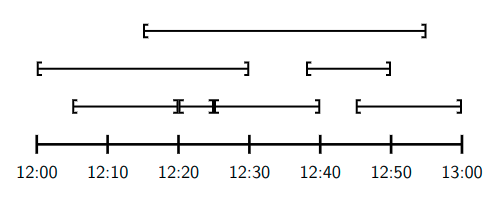
\includegraphics[scale=.5]{graph-satellite.png}
\end{center}

If we take a greedy algorithm approach to assigning these slots, we could
do something like assign the slot that finishes earliest, and then repeat
doing this until we have reached the end. For example, the slot that
finishes fastest is 12:05-12:20, so we assign this. This now removes the
ability for both 12:10-12:30 and 12:15-12:55 to be assigned, so we remove
these. This continues until we end up with something looking like this:


\begin{center}
    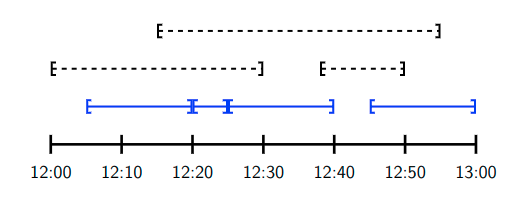
\includegraphics[scale=.5]{graph-assigned}
\end{center}

This means that we satisfy four requests (which is actually the maximum
possible, so well done us).

We can formalise this by saying that a \textbf{request} is a pair of
integers $(s,f)$ with $0 \le s \le f$.

\newpage
The algorithm that we're left with is this:
\begin{lstlisting}
public sub greedySchedule
    sort R
    for each i in {1 ... n} do
        if s_i >= lastf then
            A.append(s_i, f_i)
            lastf = f_i
        end if
    next
end sub
\end{lstlisting}

Now, we need to prove that the output is actually a \textbf{compatible
subset} of R. This is sort of intuitive because the set we added doesn't
break compatibility, since $s \ge$ \lstinline|lastf| and \lstinline|lastf|
is the latest finish time that's already in $A$.

We can formalise this with a loop invariant. At the start of the $i$th
iteration, we see that
\begin{itemize}
    \item $A$ contains a compatible subset $\{(S_1,F_1), \dots,
        (S_t,F_t)\}$ of R.
    \item \lstinline|lastf| = $\max(\{0\} \cup \{F_j : j \le t\})$ 
\end{itemize}

The base case ($i=0$) is immediate because $A = []$. The induction step is
that $A$ was compatible at the start of the iteration, and therefore if we
append a pair $s_i,f_i$ to $A$ then $s \ge $ \lstinline|lastf| $\ge F_j$
for all $f \le t$. This means that $(s_i,f_i)$ is compatible with $A$.



\end{document}
